\section{Simulation}
The objective of the simulation model is to predict the conditions under which the coincidence approach achieves greater accuracy of the transmittance than the conventional approach. The analytical formulas for calculating the variance of both approaches were given in \autoref{eq:VarianceTransExplCoinc} and \ref{eq:VarianceTransExpl}. The experiments showed that in \autoref{eq:VarianceTransExplCoinc} the variance of the coincidences and accidentals can be approximated by their mean value. The same holds true for the noise in \autoref{eq:VarianceTransExpl}, while the variance of the total counts is approximated by the mean value multiplied by a factor of 2.2. This factor results from single-photon statistics in the idler arm, which were measured experimentally. For the following analysis, it is also assumed that the presence of the sample does not change the dark counts of the detectors. \newline
There are six free parameters that need to be set in order to determine any values for both formulas:
\begin{itemize}[topsep=0pt, partopsep=0pt, itemsep=1.5pt, parsep=0pt, leftmargin=3em]
	\item $\eta_{\text{idl}}$: efficiency of the idler arm
	\item $\eta_{\text{sig}}$: efficiency of the signal arm
	\item $R_{\text{idl}}$: photon rate in the idler arm
	\item $R_{\text{noise,idl}}$: noise rate in the idler arm
	\item $R_{\text{noise,sig}}$: noise rate in the signal arm
	\item $T$: transmittance of the sample 
\end{itemize}
The idea of the simulation model is to select one of the six parameters and perform a sweep over a specified range to observe its impact on the variance of the transmittance in both approaches. The following analysis is not investigating the influence of all six parameters, but is restricted to the efficiencies of both arms !only signal! and the ratio of the noise rate to the photon rate in the idler arm. \newline
To determine the effect of the noise-to-signal ratio on the variance of the transmittance, the noise rate in the idler arm was varied between zero and one hundred times the photon rate. An overview of all six parameters is shown in \autoref{tab:SimParam}.
\begin{table*}
	\centering
	\ra{1.2}
	\begin{tabular}{@{}l@{\hspace{50pt}}lll@{}}
		\toprule[1.5pt]
		\textbf{Parameter} &  \textbf{$R_{\text{noise,idl}}$ sweep}   & \textbf{$\eta_{\text{sig}}$ sweep} & \textbf{$R_{\text{idl}}$ sweep}\\
		\midrule
		$\eta_{\text{idl}}$ (\%) & 0.09 & 0.09 & 0.09 \\
		$\eta_{\text{sig}}$ (\%) & 2.6 & 0 - 25 & 2.6 \\
		$R_{\text{idl}}$ (kHz) & 10 & 10  & 3 - 100 \\
		$R_{\text{noise,idl}}$ (kHz) & 10 - 1000  & 1000 & 1000\\
		$R_{\text{noise,sig}}$ (Hz) & 30 & 30 & 30 \\
		$T$ (1) & 1 & 1 & 1\\
		\bottomrule[1.5pt]
	\end{tabular}
	\vspace{1em}
	\caption{Overview of the simulation parameters for the different analysis scenarios}
	\label{tab:SimParam}
\end{table*}\newline
The results of sweeping the noise rate in the idler arm are shown in \autoref{fig:SimSNR}. As can be seen, for noise-to-signal ratios smaller than fifteen, the conventional approach results in smaller transmittance variance. However, as the noise increases, the variance of the transmittance increases for both approaches, and the coincidence approach's slope is smaller than the conventional approach's. Consequently, for noise-to-signal ratios greater than twenty, the coincidence approach shows smaller variance. One reason for this behavior may be that using a second arm with its imperfect efficiency lowers the overall accuracy when the noise rate is low. However, if the noise-to-signal ratio increases, the conventional approach becomes less precise because it cannot distinguish between photons that originate from a pair or from background counts. Therefore, in a scenario with a high noise-to-signal ratio, the coincidence approach offers an advantage in terms of transmittance accuracy because it can distinguish between real photon pairs and noise.
\begin{figure}[b!]
	\centering
	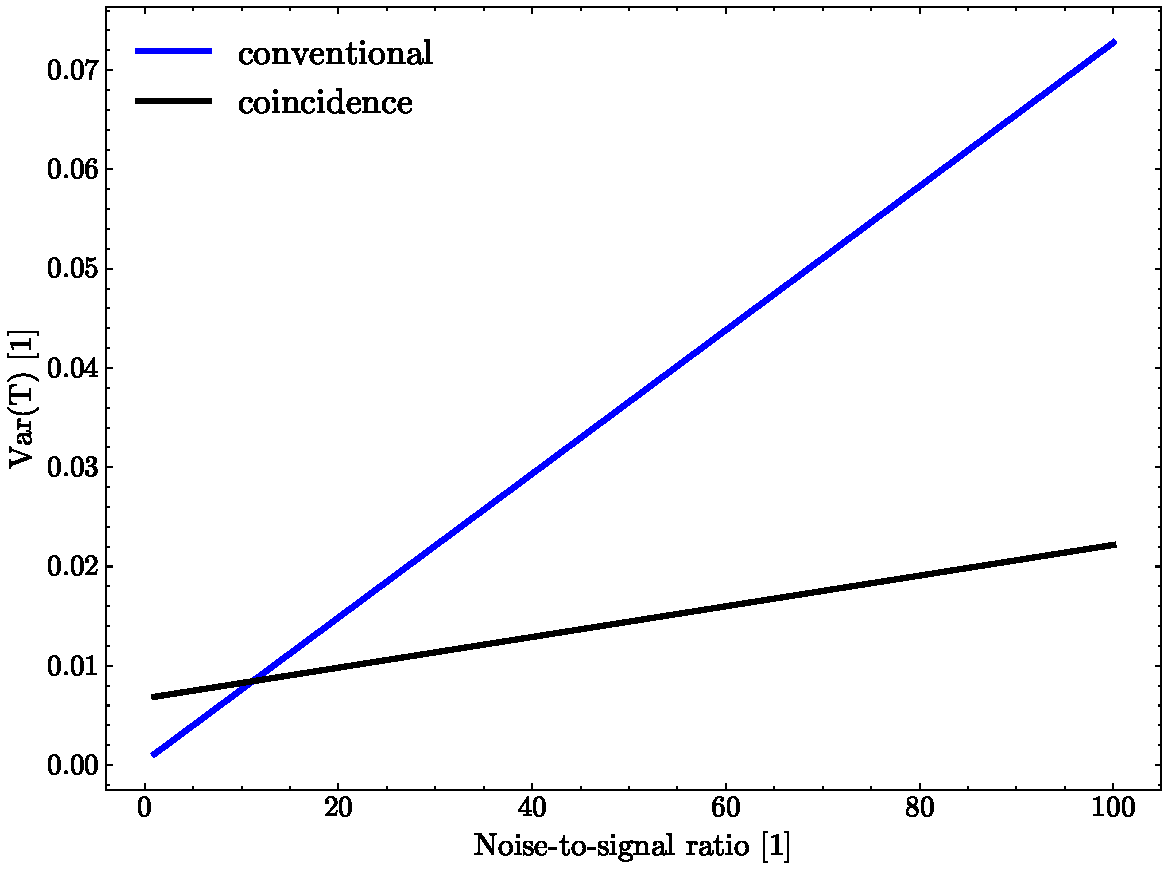
\includegraphics[width=.7\textwidth]{Images/SimulationSweepSNR.pdf}
	\caption{Variance of the transmittance as a function of the noise-to-signal ratio}
	\label{fig:SimSNR}
\end{figure}\newline
In the second analysis, the efficiency of the signal arm varied from zero to 25 percent. The values of the other parameters are listed in \autoref{tab:SimParam}. As can be seen from the results in \autoref{fig:SimEffSig}, for a signal efficiency lower than one percent, the conventional approach results in lower variance than the coincidence approach. One reason for this may be that, with low signal efficiency, many coincidence counts remain undetected, resulting in lower transmittance accuracy. As the signal efficiency increases, the variance of the transmittance decreases for the coincidence approach because it depends quadratically on the reciprocal of the efficiency. For the conventional approach, the variance of the transmittance remains constant because the signal arm does not exist in this setup. Therefore, if the signal arm efficiency is greater than one percent, the coincidence approach is expected to provide more accurate results than the conventional approach.
\begin{figure}[tb!]
	\centering
	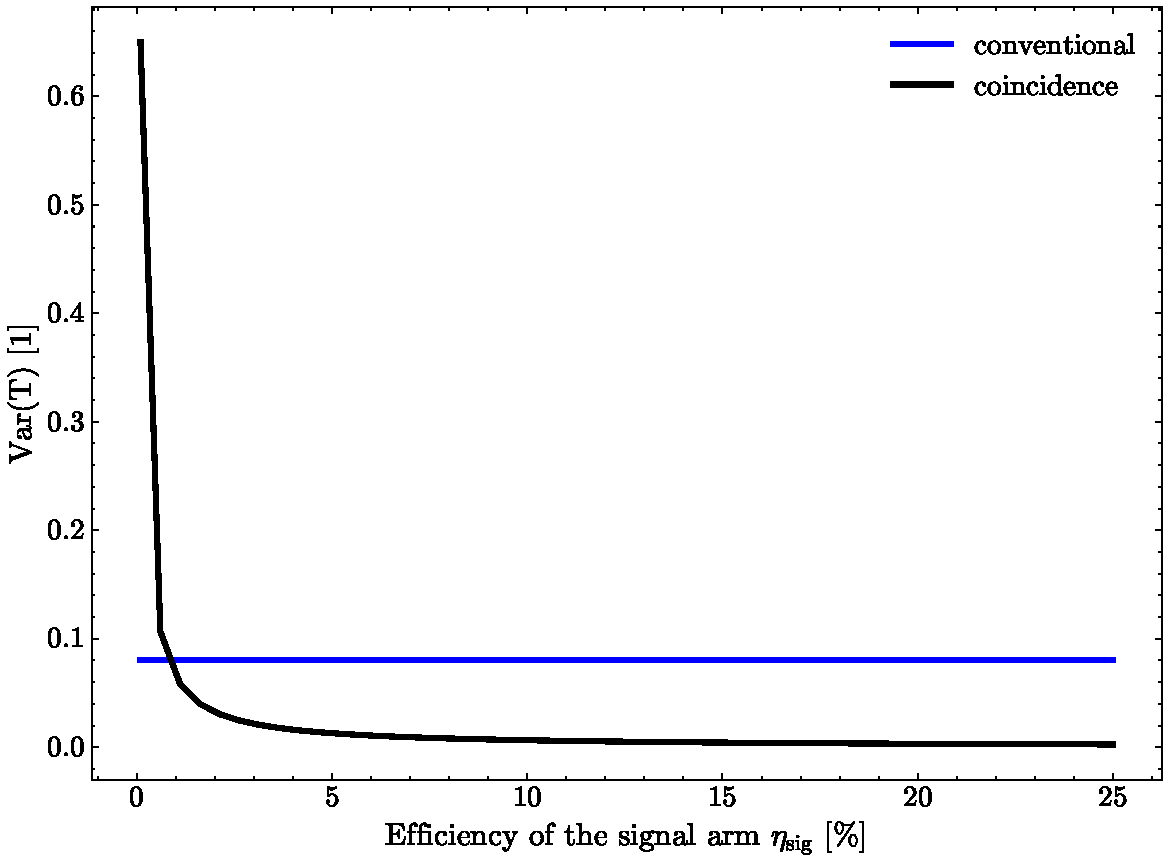
\includegraphics[width=.7\textwidth]{Images/SimulationSweepEffSig.pdf}
	\caption{Variance of the transmittance as a function of the efficiency in the signal arm}
	\label{fig:SimEffSig}
\end{figure}\newline
In the third analysis, the rate of detected photons in the idler arm was varied between three and one hundred kilohertz. The values of the other five parameters are shown in \autoref{tab:SimParam} and the results of the analysis are displayed in \autoref{fig:SimRateIdl}. It can be seen that for photon rates lower than twenty kilohertz the coincidence approach shows a smaller variance of the transmittance compared to the conventional approach, while for higher count rates both show similar results. One reason for this may be that at low photon rates the noise rate of one megahertz is comparably high and hence the conventional method cannot distinguish photons originating from a pair and dark counts. Therefore, the coincidence approach offers an advantage in terms of precision of the transmittance. With increasing count rate the difference between both methods becomes smaller as the influence of the noise rate decreases. 
\begin{figure}[tb!]
	\centering
	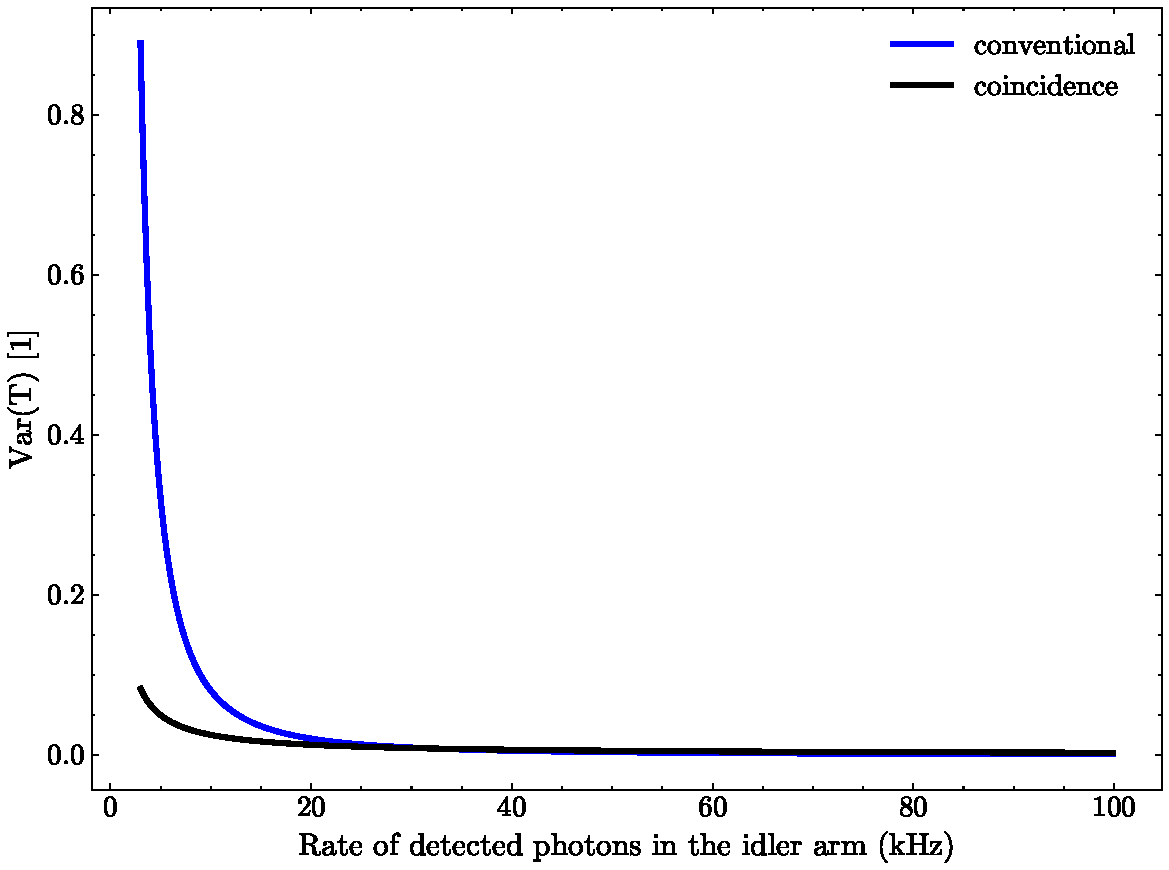
\includegraphics[width=.7\textwidth]{Images/SimulationSweepRateIdl.pdf}
	\caption{Variance of the transmittance as a function of the photon rate in the idler arm}
	\label{fig:SimRateIdl}
\end{figure}
\begin{comment}
	\begin{table*}
		\centering
		\ra{1.2}
		\begin{tabular}{@{}l@{\hspace{50pt}}l@{}}
			\toprule[1.5pt]
			\textbf{Parameter}    & \textbf{Value}  \\
			\midrule
			$\eta_{\text{idl}}$ & 0.09 \% \\
			$\eta_{\text{sig}}$ & 2.6 \% \\
			$R_{\text{idl}}$ & 10 kHz\\
			$R_{\text{noise,idl}}$ & 10 - 1000 kHz\\
			$R_{\text{noise,sig}}$ & 30 Hz\\
			$T$ & 1 \\
			\bottomrule[1.5pt]
		\end{tabular}
		\vspace{1em}
		\caption{Simulation parameters of the SNR sweep}
		\label{tab:SimSNR}
	\end{table*}
	
	\begin{table*}
		\centering
		\ra{1.2}
		\begin{tabular}{@{}l@{\hspace{50pt}}l@{}}
			\toprule[1.5pt]
			\textbf{Parameter}    & \textbf{Value}  \\
			\midrule
			$\eta_{\text{idl}}$ & 0.09 \% \\
			$\eta_{\text{sig}}$ & 0 - 25 \% \\
			$R_{\text{idl}}$ & 10 kHz\\
			$R_{\text{noise,idl}}$ & 1 MHz\\
			$R_{\text{noise,sig}}$ & 30 Hz\\
			$T$ & 1 \\
			\bottomrule[1.5pt]
		\end{tabular}
		\vspace{1em}
		\caption{Simulation parameters of the signal efficiency sweep}
		\label{tab:SimEffSig}
	\end{table*}
\end{comment}